%
%  $Description: Survey on Orchestration$
%

\documentclass[10pt,twocolumn]{article}
\usepackage{times,mathptmx,fullpage}
% Allows you to put literal text into your document without having LaTeX try to interpret it.
\usepackage{verbatim}
% Sorts citations numerically and "combines" adjacent ones
\usepackage{cite}
% Allows you to individually label subfigures in a multi-part figure
\usepackage{subfigure}
% Allows the definition of macros that are smart about adding space after text in a macro
\usepackage{xspace}
% To use external images
\usepackage{graphicx}

% Redefine the percentage of the page that can be used for floats (figures, tables, etc.)
\renewcommand\floatpagefraction{.9}
\renewcommand\dblfloatpagefraction{.9}
\renewcommand\topfraction{.9}
\renewcommand\dbltopfraction{.9}
\renewcommand\bottomfraction{.9}
\renewcommand\textfraction{.1}
\setcounter{totalnumber}{10}
\setcounter{topnumber}{10}
\setcounter{dbltopnumber}{10}
\setcounter{bottomnumber}{10}

% Set values for float separation from text
\setlength{\floatsep}{1.5ex plus1.0ex minus 0.2ex}
\setlength{\dblfloatsep}{1.5ex plus1.0ex minus 0.2ex}
\setlength{\textfloatsep}{1.5ex plus1.0ex minus 0.2ex}
\setlength{\dbltextfloatsep}{1.5ex plus1.0ex minus 0.2ex}
\setlength{\abovecaptionskip}{0.5ex}
\setlength{\belowcaptionskip}{0.5ex}

% Don't allow widows or clubs - single lines at the start/end of a column
\widowpenalty=10000
\clubpenalty=10000

\newcommand{\latex}{\LaTeX\xspace}
\pagestyle{plain}

%-------------------------------------------------------------------------
\begin{document}

\title{A Survey on Virtual Machine and Container Orchestration}

\author{
Aneesh Neelam \\
\textit{Univ. of California, Santa Cruz} \\
\textit{aneelam@ucsc.edu}
}

\maketitle
\thispagestyle{empty}

\begin{abstract}

  Data center administrators and site reliability engineers create virtual machines or containers to run their applications, with desired redundancy requirements and automated coordination between the replicas.
  This is called the orchestration of the various computing, storage and network resources of the data center.
  To automate the orchestration process, different tools have been developed in the past couple of decades.
  Each tool was designed differently, with different intents and priorities but they also have a lot in common.
  This survey is on the various orchestration tools available to data center administrators, site reliability engineers and software engineers;
  and aims to be a comprehensive guide that helps data center managers in choosing the cloud platform and the orchestration tool.

\end{abstract}

%-------------------------------------------------------------------------
\section{Introduction}

With the advent and proliferation of virtualization, computing as a service has taken off.
Now there are multiple cloud service providers such as Google Cloud, Amazon Web Service, Microsoft Azure, etc.
The operators of these cloud services typically have their own data centers, each consisting of thousands of physical machines connected via a high speed and very low latency network such as Infiniband (IB) ~\cite{intro_infiniband}.
Data center operators use various tools to automate the process of management, provisioning and scaling the resources for their customers.

Orchestration tools have been developed to ease the operation of a data center.
Tools such as OpenStack's Heat have been used to manage Linux kernel virtual machines ~\cite{openstack}.
There are many other such tools such as Chef and Ansible for virtual machines ~\cite{chef, ansible}.
Container Orchestration tools such as Docker Swarm, Kubernetes, Mesos have been developed to manage containers on mostly Linux machines ~\cite{docker_swarm, kubernetes, mesos}.
In this survey, however, we shall focus more on the orchestration of containers than virtual machines.

Using these orchestration tools, data center operators can boot up virtual machines or containers on the physical machines, and control the entire the data center as a single entity, provision the necessary resources, and deploy and managing applications.
These orchestration tools can also be used to automate replication of processes, fault tolerance, failure detection and recovery, live migration of processes or entire virtual machines between physical machines, and also set up coordination between the processes to make the development of applications for the distributed system easier ~\cite{live_migration, xen}.
Some orchestration tools also enforce quotas for processes, ensure that Service-level agreements are adhered to and can also be used to keep track of the overall resource utilization and power consumption of the data center.

In this survey, the performance of these orchestration tools shall be compared.
Also, these orchestration tools may also have different guarantees of tolerance when there is a failure or network partition.
According to the CAP theorem, only two out of three: presence of network partitions, availability and consistency can be guaranteed by any distributed system ~\cite{CAP_theorem}.
In which case, there may be different methods the orchestration tools employ for error recovery and maintain high reliability, offering various combinations of two out of the three things for applications to easily support.

In the next section, we shall see some of the past work on virtualization, the use of virtual machines and containers, and the approaches taken by the different virtualization technologies to enforce isolation between applications.
In Section 3, we shall describe how virtual machines and containers controlled by the various orchestration tools.
In Section 4, we analyze the limitations, evaluate the performance and ease of use, and also compare the different approaches they take for coordination and failure.
We then discuss possible future work in the field in Section 5, and we then conclude in Section 6.

\begin{figure*}
  \centering
    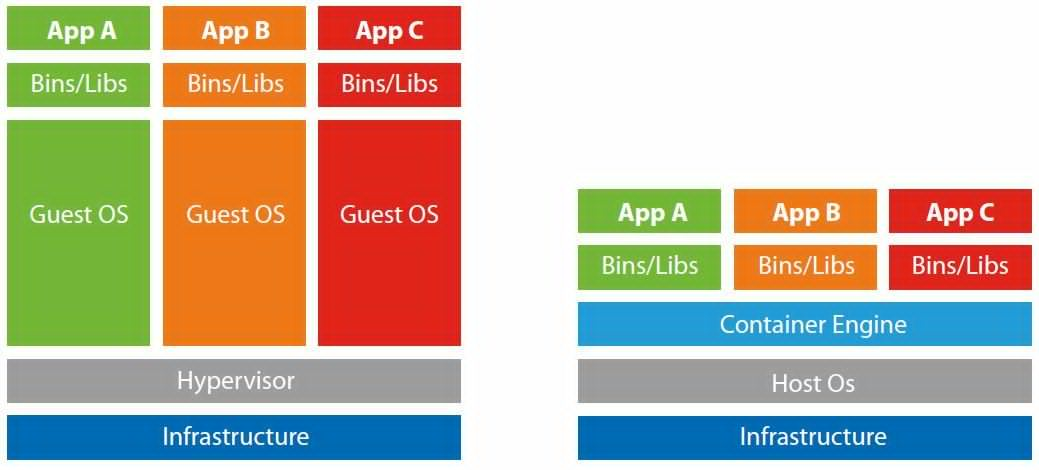
\includegraphics[width=\textwidth]{container_vm}
    \caption{Differences between Virtual Machines and Containers ~\cite{intro_containerisation}}
  \label{overflow}}
\end{figure*}

%-------------------------------------------------------------------------
\section{Background}

The increasing proliferation and popularity of virtualization technology were necessary for the data center, and cloud service providers to thrive.
Virtual machines allowed for running more isolated virtual operating systems or applications on a lesser number of physical machines.
The use of these virtual machines could be leased out to third-parties, providing a revenue stream for people who may have powerful physical machines but are unable to push them to their full potential.
Consequently, cloud computing has made the concept of computing as a utility possible ~\cite{berkeley_cloud}.
Virtualization, in this context, is the task of creating virtual hardware and running actual operating systems and applications on top of them.
Each of these virtual machines is isolated and independent from one another and are managed by a hypervisor that is running on the physical hardware or the host operating system ~\cite{xen}.

Virtualization technology is now decades old, with every major operating system that runs on servers having built-in virtualization support without the need for a third-party hypervisor.
For example, the Linux kernel has KVM and Microsoft Windows Server has Hyper-V.
Both also have well-documented endpoints for various front-ends to interface with, providing data center operators and server administrators with many tools to automate and manage their machines.

A similar development is going on with containers on these operating systems as well. Like Cgroups in the Linux kernel, Hypervisor.framework in Apple macOS and Hyper-V in Microsoft Windows.
Container engines that provide a cross-platform frontend but make use of the respective container support structure in the host operating system have been developed, of which the most prominent is Docker ~\cite{intro_docker}.

Virtual machines are a complete hardware virtualization, and there is a full-fledged guest operating system on which applications are run. Virtual machines enable the use of legacy applications that require legacy operating systems that only run on legacy hardware.
The necessary legacy hardware can be emulated by the hypervisor, allowing the unmodified operating systems and applications to be run.
There is also paravirtualization where a significant increase in performance can be achieved with some changes to the guest operating system, but it still does not entail modifying the application ~\cite{xen}.

However, containers provide the isolation of virtual machines without much of the overhead. There is no guest operating system, and the host kernel itself enforces isolation ~\cite{intro_containerisation}.
However, that would also mean that the applications would have to be able to execute directly on the host operating system.
Hence, this technique may not be used to run legacy applications.

Figure 1 shows the differences between virtual machines and containers ~\cite{intro_containerisation}.
Containers, with none of the overhead of virtual machines and the lack of guest operating systems, can be used to start up many orders of magnitude number of applications on the same host kernel.
Containers are still new, however, and the implementation in the various operating system kernels may have bugs that compromise this isolation.

Orchestration tools for managing virtual machines and containers on many physical machines in a cluster have been developed.
Tools for virtual machines that we shall evaluate in this survey include OpenStack ~\cite{openstack}, Chef ~\cite{chef} and Ansible ~\cite{ansible}.
Some of the tools for containers we shall cover in this survey are Docker Swarm ~\cite{docker_swarm}, Kubernetes ~\cite{kubernetes}, Mesos ~\cite{mesos}.

%-------------------------------------------------------------------------
\section{General Comparison}

As we have seen in the previous section, virtual machines are full-fledged operating systems, each that contain their own set of libraries and run applications.
These virtual machines are all isolated and are managed by the hypervisor running on the corresponding physical machine.
Orchestration tools such as OpenStack Heat ~\cite{openstack} or Ansible ~\cite{ansible} or Chef ~\cite{chef} can be used to manage all the hypervisors of a cluster of physical machines, thereby controlling the entire data center as one entity.

\begin{figure}[thpb]
  \centering
      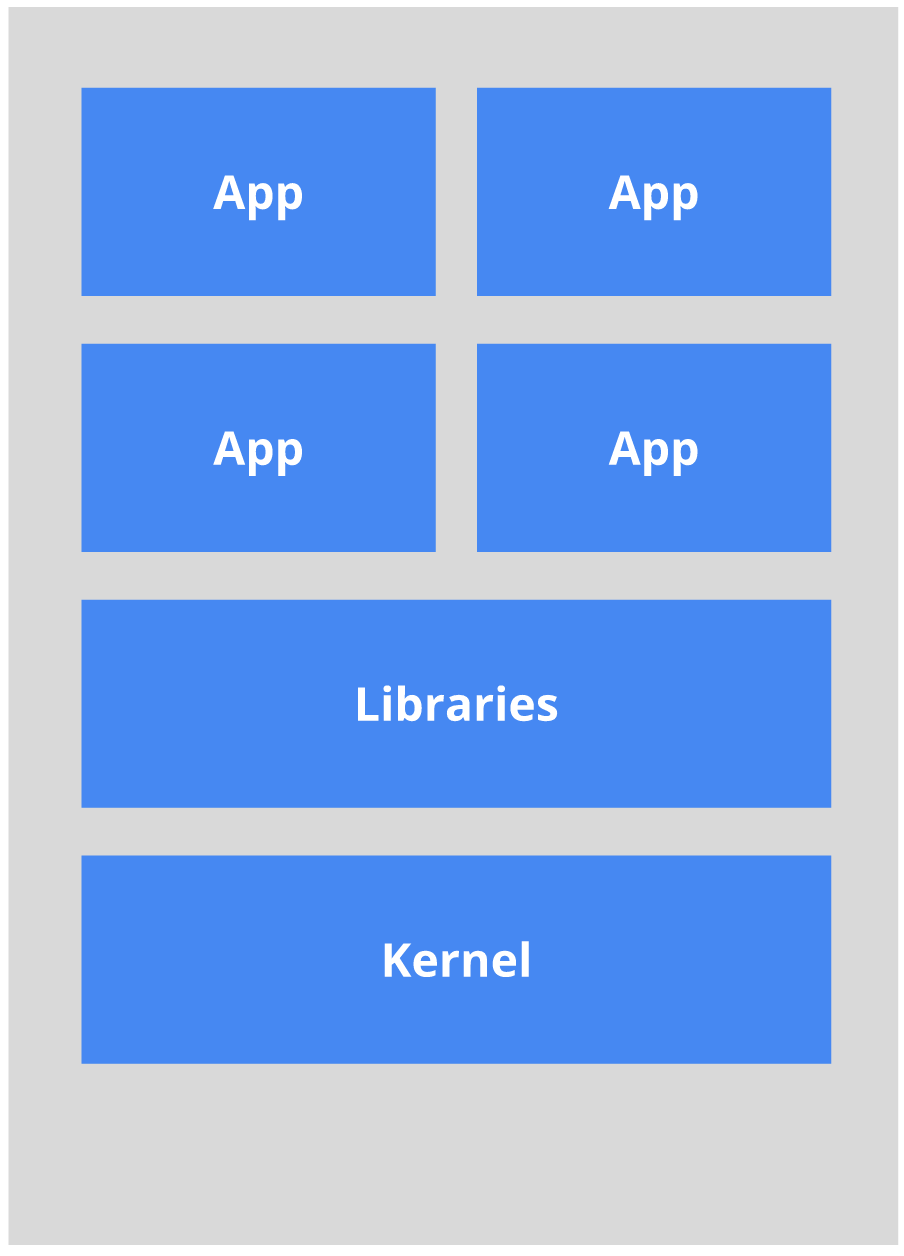
\includegraphics[width=\columnwidth]{native_app_libs}
    \caption{Applications running natively on OS with shared libraries ~\cite{container_shared_lib}}
    \label{fig:native_app_libs}
\end{figure}

However, containers have one key advantage greatly increased their popularity, and that is their significantly lower overhead when compared to virtual machines.
This is especially true when two or more applications link with different versions of libraries, but the operating system provides shared libraries that are a single version as depicted in Figure 2 ~\cite{container_shared_lib}.
One can run the applications in different contexts by running each one in its own virtual machine, but the overhead of virtualization is very high.
Containers allow the kernel-level isolation of applications \textbf{and their libraries}.
Figure 3 illustrates the use of containers for this use case ~\cite{container_shared_lib}.

\begin{figure}[thpb]
  \centering
      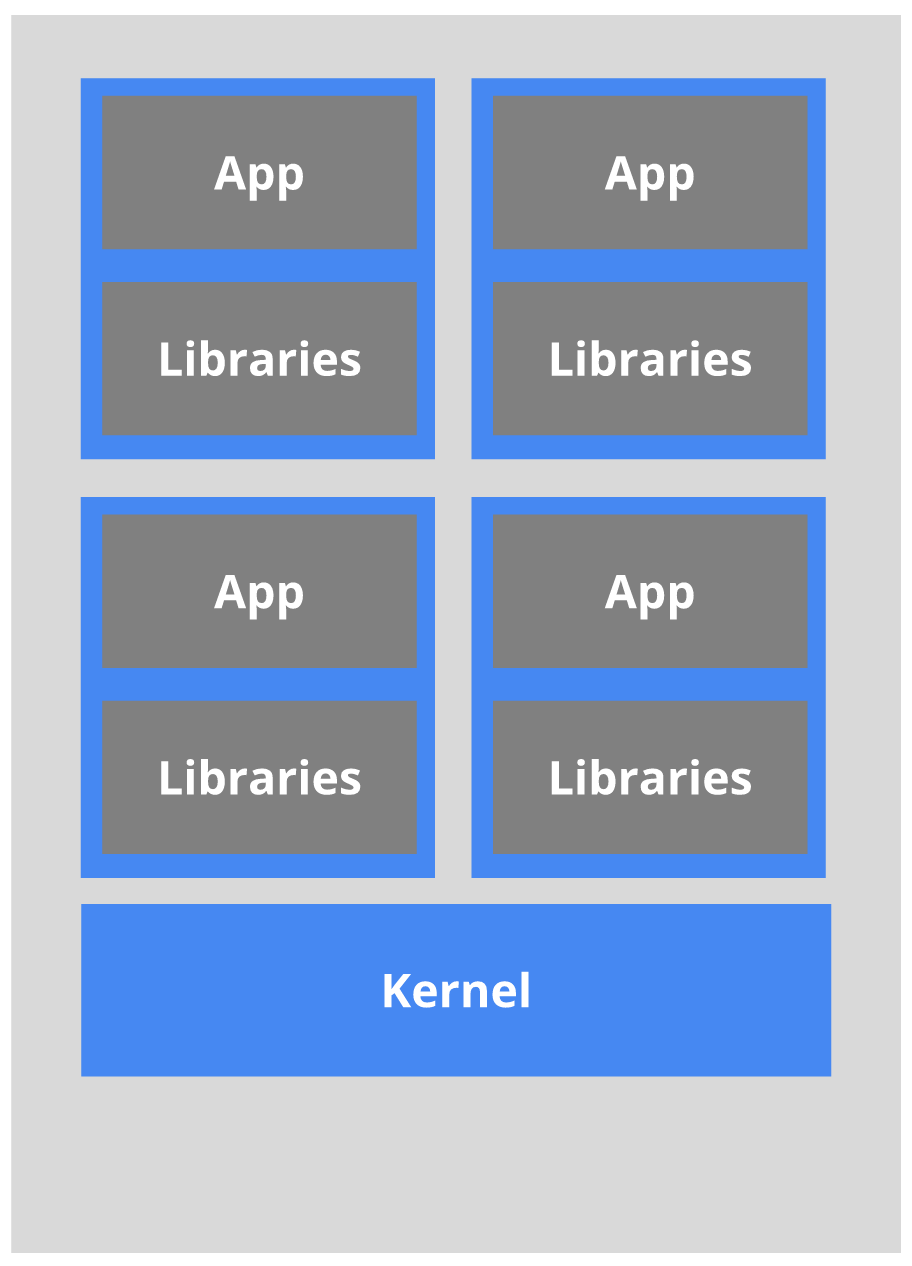
\includegraphics[width=\columnwidth]{container_app_libs}
    \caption{Containers of applications and libraries running on OS ~\cite{container_shared_lib}}
    \label{fig:container_app_libs}
\end{figure}

Therefore, data center operators use a combination of virtual machines and containers on their physical clusters.
Hence, orchestration tools for both are used in most data centers.

\begin{figure*}
  \centering
    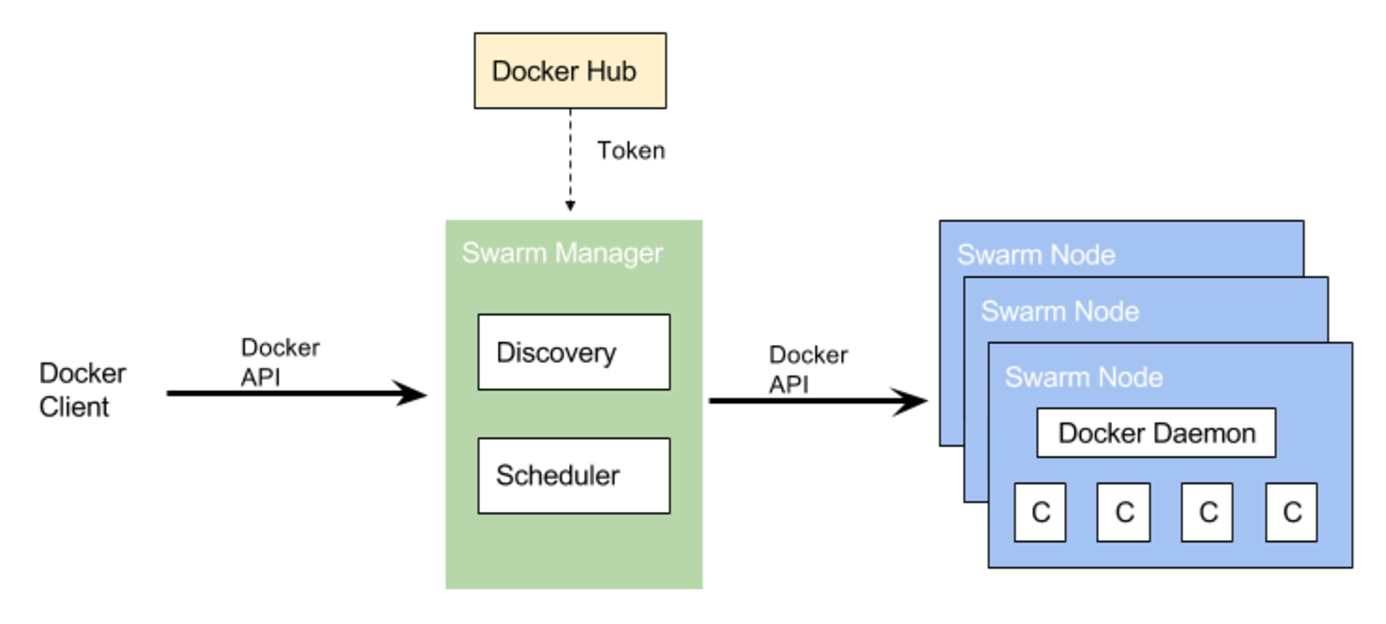
\includegraphics[width=\textwidth]{docker_swarm}
    \caption{Overview of Docker Swarm ~\cite{platform9_dockerswarm_kubernetes}}
  \label{overflow}}
\end{figure*}

\subsection{Virtual Machine Orchestration}

As mentioned previously in this paper, the use of virtual machines is still necessary when a full-fledged guest operating system is needed.
This is particularly the case when running legacy applications that require legacy operating systems and legacy hardware.
But advances in automation and orchestration can be applied to machines that emulate legacy hardware as well.

Ansible is an automation tool for managing massive physical clusters and deploying applications on them ~\cite{ansible}.
However, Ansible does not control the native operating system running on the physical server, but the virtual machines and applications running on it.
It is made up of many components, not all relevant for this survey.
We shall focus on the orchestration capabilities of Ansible.
An administrator can execute hundreds or thousands of virtual machines, specifying an operating system and application image with a complex network configuration set up between them.
Configuration is predetermined by the administrator, written into the config file(s) and specified when running the orchestration tool.

Chef works similarly to Ansible ~\cite{chef} and orchestrates only the virtual machines and applications.
Like Ansible, Chef also follows the master-slave architecture as depicted in Figure 5 ~\cite{chef_overiew}.
Chef server contains the information about the Chef clients, which are the other nodes in the cluster.
The Chef clients pull the specified configuration from the server sets up the nodes in the cluster.
Application developers can make use of the Chef Developer Kit to quickly design and build the configuration and the applications.
This configuration is then pushed to the Chef server.

\begin{figure}[thpb]
  \centering
      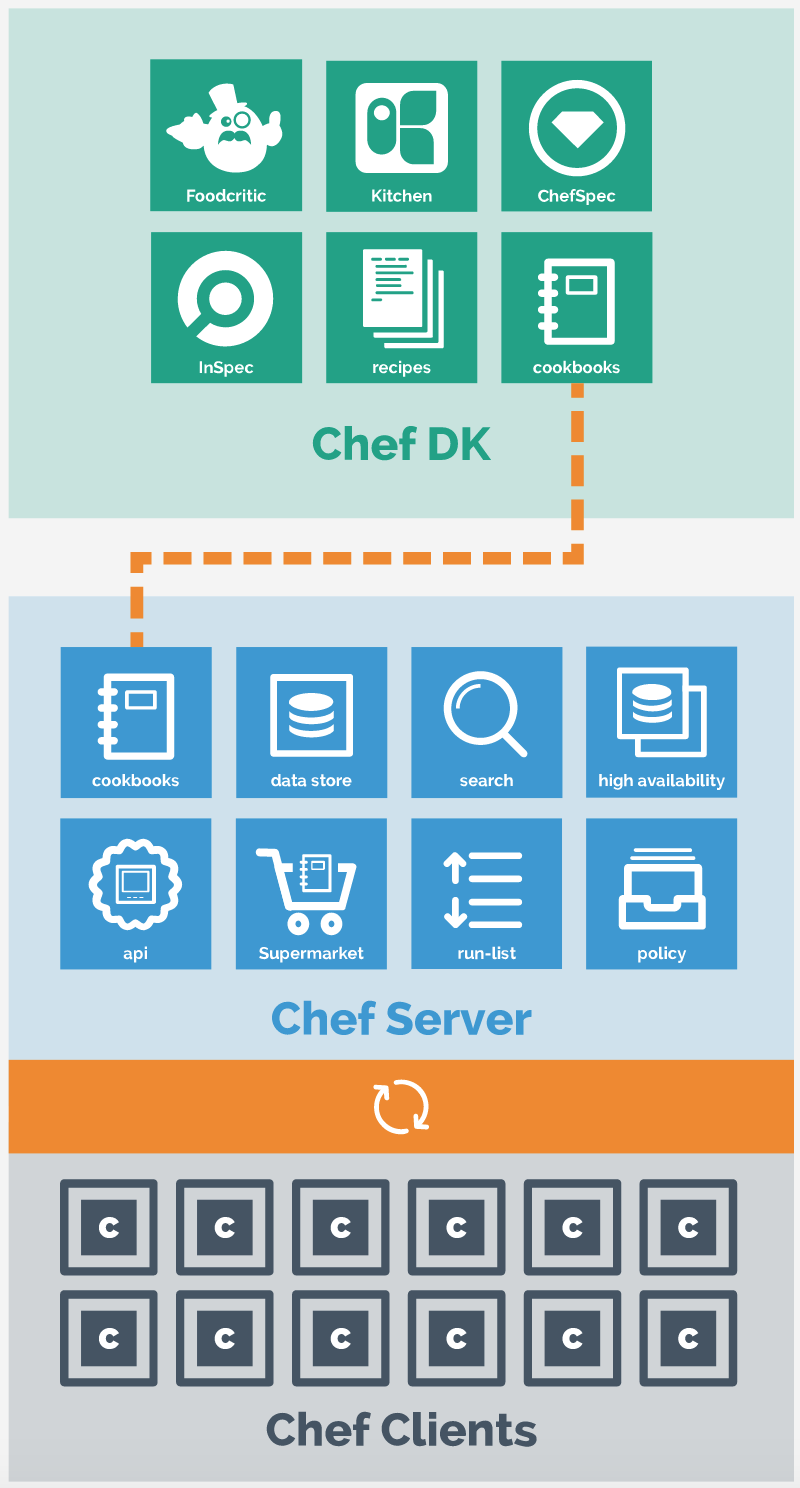
\includegraphics[width=\columnwidth]{chef}
    \caption{Overview of Chef ~\cite{chef_overview}}
    \label{fig:chef}
\end{figure}

OpenStack Heat is another orchestration tool that can be used to manage bare physical servers ~\cite{openstack}.
Administrators can describe their cluster and specify the applications that are desired to run using a declarative language.
It can be used in conjunction with Ansible or Chef to control the entire data center infrastructure.

\subsection{Container Orchestration}

We shall compare Docker Swarm ~\cite{docker_swarm}, Kubernetes ~\cite{kubernetes} and Apache Mesos ~\cite{mesos}.
Docker Swarm, Kubernetes, and Mesos all have a master-slave architecture, where a small number of manager nodes monitor the rest of the cluster ~\cite{docker_swarm, kubernetes, mesos}.

Docker Swarm is an extension of the Docker container engine itself and is trivial to set up.
The Docker Container Engine must be installed on the nodes of the cluster, each of which must also be associated with a discovery service.
The discovery service backend is what the swarm manager(and their replicas) and the nodes use to authenticate themselves as members of the swarm cluster.
The swarm manager is the one that controls the other nodes of the cluster.
Replicas of the swarm manager take over in the case of a failure. ~\cite{docker_swarm}.
Third party tools that maintain high availability of the swarm manager can be integrated into this setup ~\cite{platform9_dockerswarm_kubernetes}.

One of the key advantages of Docker Swarm is how it can be interfaced with using the same Docker API.
As depicted in Figure 4, the same Docker API that is used by so many frontends is the same one used to control Docker Swarm ~\cite{platform9_dockerswarm_kubernetes}.

Kubernetes is an orchestration tool developed by engineers at Google.
Like Docker Swarm, Kubernetes also works with the Docker Container Engine ~\cite{kubernetes}.
It was originally for internal use only and was designed to orchestrate the use of their internal cluster, Borg ~\cite{borg}.
But with the advances in containerization and the increasing use of containers to isolate applications, Google gave away some of the source code behind Kubernetes ~\cite{kubernetes_github}.
As illustrated in Figure 6, Kubernetes has a master-slave architecture ~\cite{platform9_dockerswarm_kubernetes}.
Pods are groups of containers that run on the nodes in the cluster ~\cite{kubernetes}.

\begin{figure}[thpb]
  \centering
    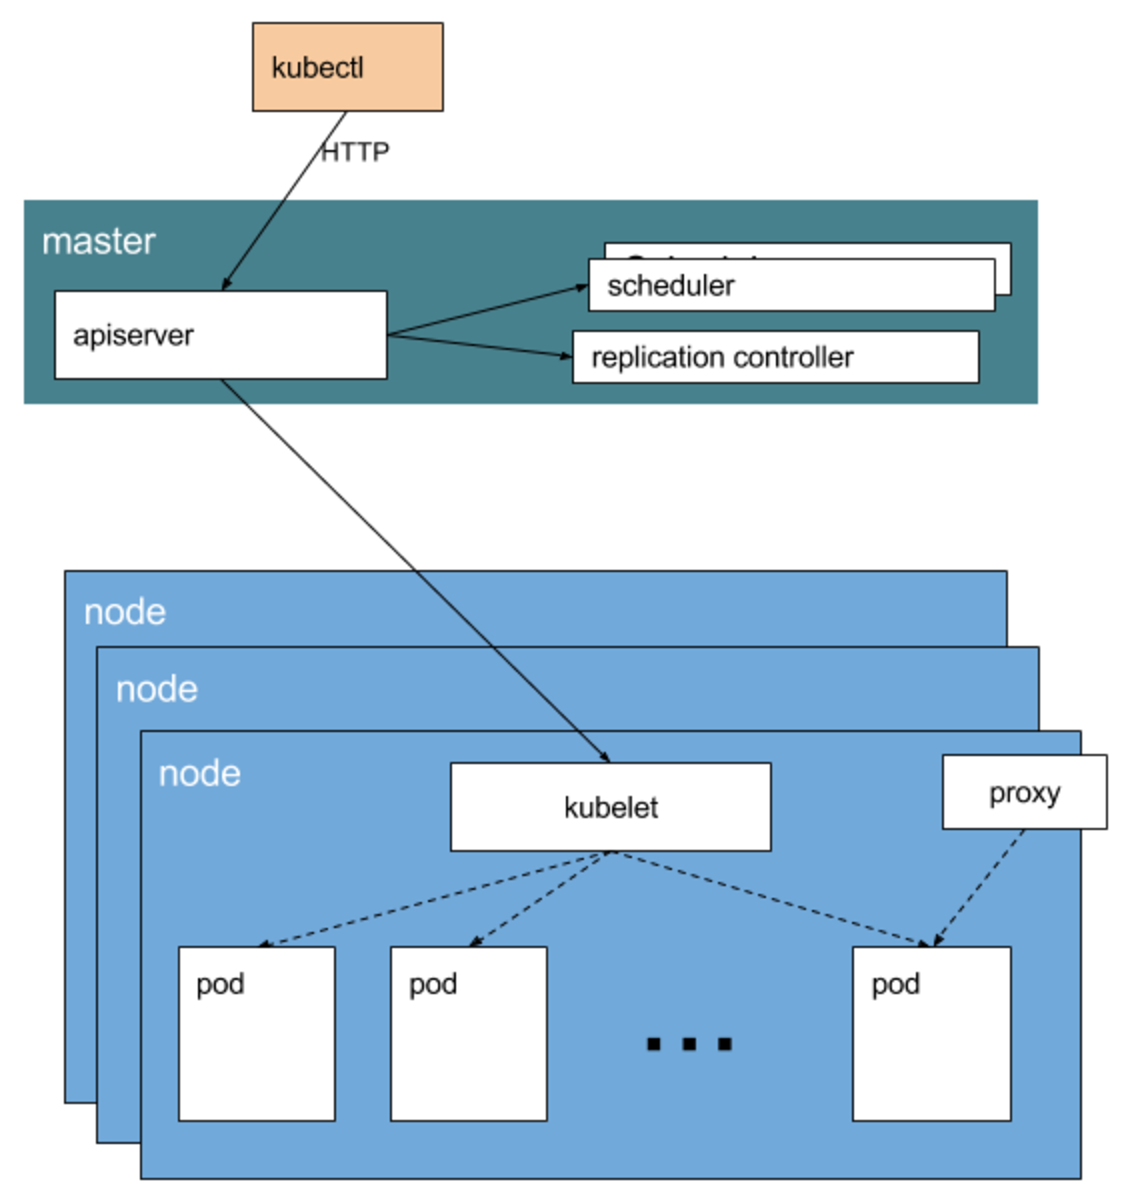
\includegraphics[width=\columnwidth]{kubernetes}
    \caption{Overview of Kubernetes ~\cite{platform9_dockerswarm_kubernetes}}
  \label{fig:kubernetes}}
\end{figure}

Mesos is another orchestration tool that manages containers ~\cite{mesos}.
Mesos, like Docker Swarm and Kubernetes, allows for data center operators to control the entire data center as a single entity.
As depicted in Figure 7, Mesos has a master-slave architecture, like Docker Swarm and Kubernetes.
The Mesos kernel runs on every node in the cluster.
This enables the interfacing between the Mesos slave nodes and the Mesos master node.
Using a coordination tool, like Zookeeper ~\cite{zookeeper}, the availability of the mesos master can be maintained by switching over to the master replicas when a master failure occurs.
Mesos has frameworks for Hadoop and MPI; that application developers can use to build and run their Hadoop or MPI jobs using Mesos ~\cite{mesos}.

\begin{figure*}
  \centering
    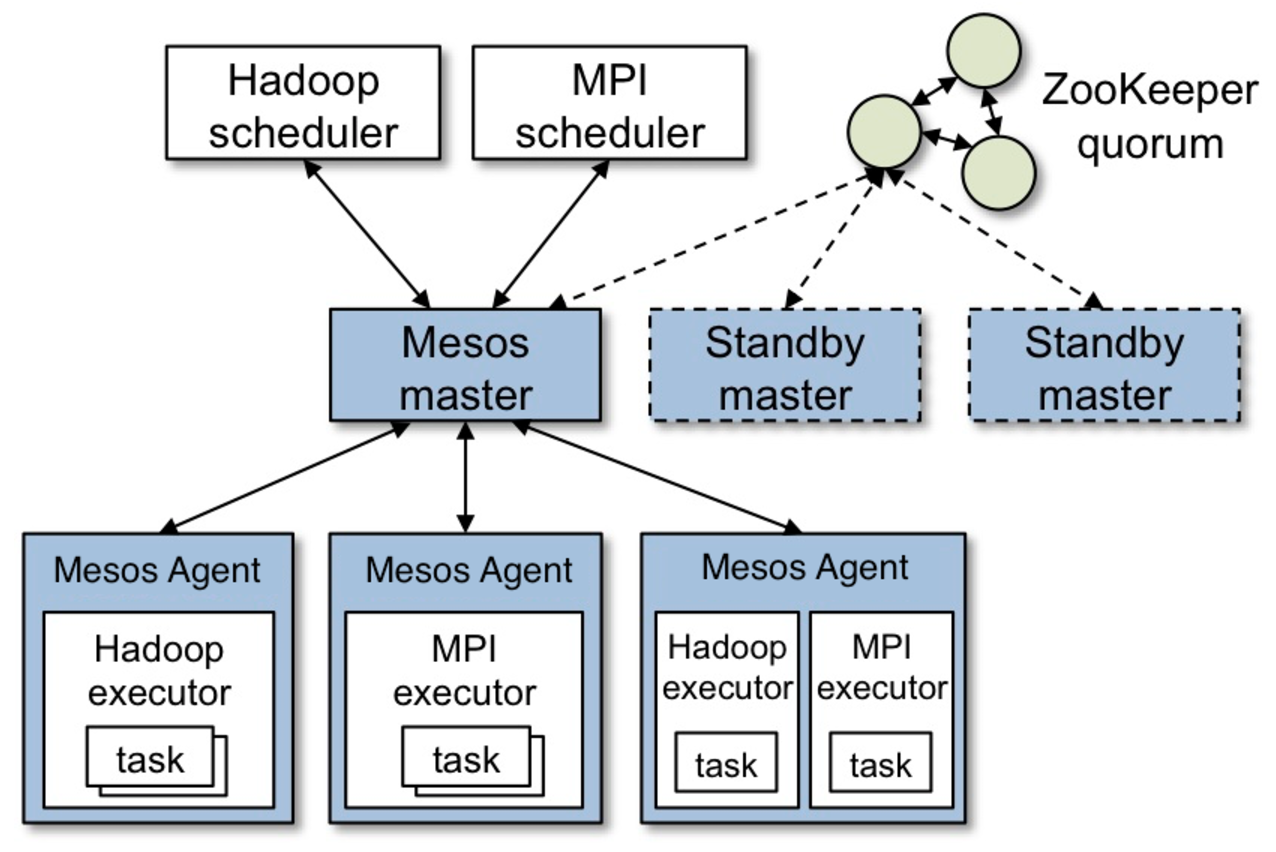
\includegraphics[width=\textwidth]{mesos}
    \caption{Mesos Architecture ~\cite{mesos}}
  \label{overflow}}
\end{figure*}

%-------------------------------------------------------------------------
\section{Evaluations}

Orchestration tools are vital for Developer Operations (DevOps).
But there is a real dearth of scholarly research work on the orchestration tools mentioned previously here.
Therefore, we have also referenced whitepapers; documentation provided to data center operators,  and performance and scalability results from benchmarking organizations ~\cite{orchestration}.
As we have already seen, Orchestration tools, for the most part, are quite similar in nature.
All of them attempt to solve some of the same kinds of problems, and some also in similar or even identical manners.

For many of the generic container use cases, one could work with Docker Swarm, Kubernetes and Mesos as all three can be configured to use the same Docker Container Engine ~\cite{docker_swarm, kubernetes, mesos}.
And since containerization is an operating system feature, all container engines would have to use the same kernel interfaces to initialize and manage containers on a particular operating system ~\cite{intro_containerisation}.
Hence, in this section, we shall be going over some of the different methods the orchestration tools use to solve problems including those of performance and scalability.
Also, we shall be comparing their ease of use, their community support and their popularity with data center operators as well as application developers.

\subsection{Performance and Scalability}

Virtual machines will obviously be slower than containers. Hence we shall not be comparing them.
However, we shall be comparing the various container orchestration tools: Docker Swarm, Kubernetes, and Mesos ~\cite{docker_swarm, kubernetes, mesos}.

The developers of Docker Swarm claim that it can scale up to tens of thousands of containers with little performance degradation, whereas Kubernetes is an order of magnitude less scalable ~\cite{docker_swarm}.
But, benchmarks have proven that Docker Swarm provides much better performance than Kubernetes ~\cite{dockerswarm_vs_kubernetes}.

\subsection{Protocols used}



\subsection{Ease of use and other advantages}

Ansible and Chef are used to manage applications running on virtual machines on physical machines in a data center ~\cite{ansible, chef}.
Both are quite similar in their use cases.
Chef is more full-fledged as it requires the use of the Chef Developer Kit to configure and describe a cluster ~\cite{chef}.

Kubernetes, Docker Swarm, and Mesos all can use same Docker Container Engine ~\cite{kubernets, docker_swarm, mesos}.
While Mesos also has support for its own Mesos Container Engine, the use of Docker Container Engine is almost ubiquitous in the container community ~\cite{intro_docker}.
The use of Docker Container Engine enables the use of the Docker repository for pulling commonly used configurations and applications on Docker.
Since the Docker community is so vast, the documentation, technical support, and compatibility are, in our opinion, in a good state.

Google engineers developed Kubernetes for their internal use.
It was originally used for building and testing internal Google code on their cluster Borg ~\cite{kubernetes, borg}.
For more than a decade, Google has been using Kubernetes successfully to orchestrate their build and test machines in their cluster.
Now with the increasing popularity of containers, Kubernetes is now available for anyone to use for their orchestration needs ~\cite{kubernetes_github}.
With Google's stamp of support and a growing community of administrators and developers, Kubernetes has become the most popular container orchestration tool ~\cite{openhub}.

Kubernetes is more fully featured than Docker Swarm or Mesos ~\cite{kubernetes}.
For example, Docker Swarm does not have a built-in monitoring agent that can also perform autoscaling of the containers based on the CPU usage or other factors.
However, external monitoring tools can be used with Docker Swarm ~\cite{docker_swarm}.
And autoscaling can be setup using external tools that interface with the Docker API.

Mesos also has support for autoscaling but is available only for Mesosphere Enterprise customers ~\cite{mesosphere}.
Therefore, an external third party tool is necessary for autoscaling in Mesos as well.
Also, the popularity of Docker Swarm and Kubernetes is eclipsing that of Mesos, driving up community usage and vendor support ~\cite{openhub}.

However, Docker Swarm exposes the same Docker APIs to data center operators ~\cite{docker_swarm}.
Hence, Docker CLI or Docker Compose ~\cite{docker_compose} can be used to design and describe multi-container applications, which are apt for distributed systems.
Docker Swarm is, therefore, the easiest to set up for data center operators.
And administrators can pick and choose their third party external tools to integrate into their container engine and orchestration tool to provide the extra features that are necessary.

\subsection{Caveats}

Some tools like Chef exhibit vendor lock-in by enforcing the use of the Chef Developer Kit.
The description of the desired configuration of the cluster and the network is written in a declarative language that cannot be easily converted to the formats used by Ansible.

Some like OpenStack follow the standard set by the community and consortium of cloud software providers.
But, OpenStack is for quickly setting up bare metal physical machines and quickly building up a data center or a cloud.
And OpenStack Heat is the component that orchestrates the setup and management of OpenStack ~\cite{openstack}.

Documentation is still extremely limited for the container orchestration tools.
Since the tools have been developed only in the past few years, some of the interfaces are not stabilized for long term use yet.
Therefore whatever frontend the data center operator uses to interface with Docker Swarm or Kubernetes or Mesos, it may quickly become incompatible with a newer release of the orchestration tool or the Docker Container Engine.

%-------------------------------------------------------------------------
\section{Future of Orchestration}

For a data center operators, cluster administrators and also distributed application developers, automation and ease of management is necessary for greater efficiency.
While the current orchestration tools have similar architectures, and also provide similar functionality, there is always scope for improvement.
Small gains in performance, scalability or even ease of use improves the efficiency of operating a distributed cluster.
Due to the scale of data centers and the cloud, small gains could translate to significant increases in performance, scalability, and significant decreases in power consumption and other costs of operations.

There is a dearth of scholarly work in this field, especially regarding the evaluation of modern container orchestration tools when it comes to performance and scalability.
However, this could be because the tools are still under continuous rapid development, trying to outdo one another.
And a paper that comprehensively evaluates them could get quickly outdated.
This is particularly the case when some of the components involved in the software infrastructure of container orchestration are also the same for different orchestration tools ~\cite{intro_docker}.

The use of virtual machine orchestration tools like Ansible and Chef shall decrease, however, as modern distributed applications are more suitable to be run in containers.
OpenStack and its orchestration component Heat shall continue to be used to set up bare metal physical machines; each one would have an operating system, and a container engine can be configured.
Container orchestration tools can then be used to describe and manage them.
However, the use of virtual machines will not entirely die out, as detailed in the next section.

\subsection{Use of Virtual Machines}

Container Engines running on virtual machines is preferable over running container engines natively over physical machines.
This is because live migration of virtual machines is easier and more straightforward than a live migration of a natively running operating system ~\cite{live_migration}.
Hence, resource quotas are hit on the physical node, migration of virtual machines is performed by the hypervisor to balance the load on the physical machines.

Also, as mentioned previously, virtual machines are necessary for running legacy applications that only run on legacy operating systems and legacy hardware that are very difficult or infeasible to obtain.
A legacy distributed application would require the use of OpenStack Heat to set up the physical machines, Ansible or Chef for a virtual machine and application orchestration.
Since containers do run the application natively, albeit with kernel-level isolation, they are not suitable for running legacy applications.

%-------------------------------------------------------------------------
\section{Conclusion}

The use of orchestration tools for managing containers and virtual machines running on many physical machines is only increasing.
Orchestration tools provide one important function, and that is the automation of running distributed applications.
A distributed system consists of many processes, each running in an isolated manner in its own virtual machine or container.
It is necessary for the administrator to control and manage the entire distributed system as a single entity.

%-------------------------------------------------------------------------
\bibliographystyle{latex8}
\bibliography{orchestration}

\end{document}
